\subsection{Mechanism overview}
In conclusion, the nD-Laplace mechanism is capable of providing $\epsilon-d_x$-privacy (as well as \gls{gi}) as demonstrated in Formula \ref{theorem:nd-laplace}. The grid-nD-Laplace variant also offers the same privacy guarantee, as proven in Section \ref{section-grid-remapping}. Additionally, the density-nD-Laplace mechanism, being a post-processing step, provides an equivalent level of privacy as nD-Laplace. This equivalence extends to clustering as well.

Furthermore, it is worth noting that the use of kd-trees simplifies the complexity of these variants without compromising their privacy guarantees. Kd-trees serve as a tool to address the search complexity in handling n-dimensional data, rather than directly affecting the privacy assurances.
The following sections will provide a comprehensive framework overview and offer practical insights for its application.

\subsubsection{Flowchart}
All formulas and theories are established for 2D, 3D, and nD-Laplace, so the mechanism design applies to all three variants:
\begin{figure}[h]
  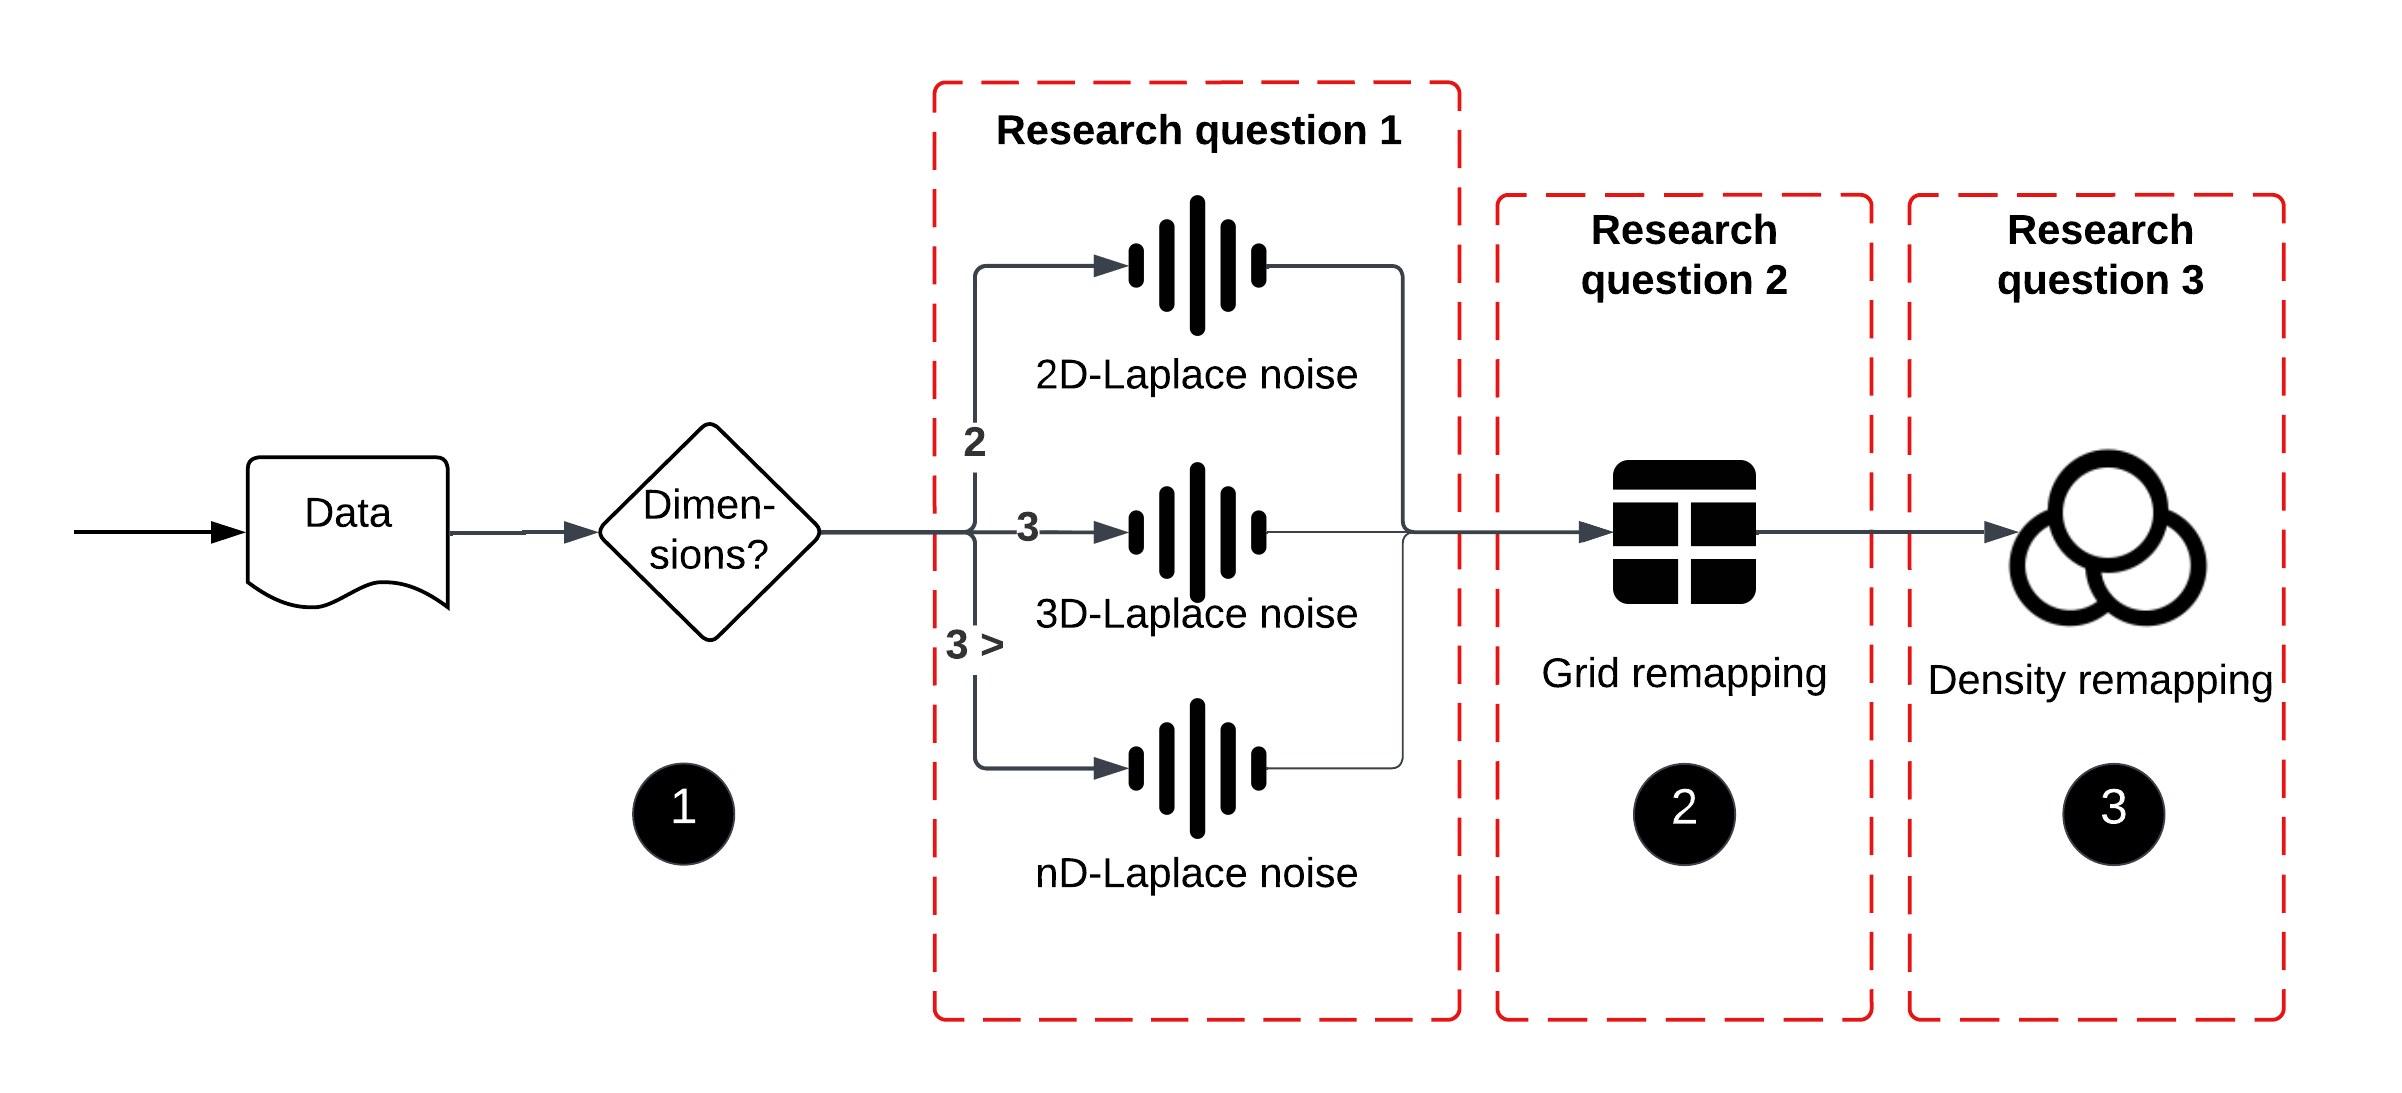
\includegraphics[width=1.1\textwidth]{TheorethicalFramework//ND-Laplace//Images/overview.png}
  \caption{Non-interactive mechanism design for nD-Laplace.}
  \label{fig:final-mechanism-design}
\end{figure}
%\todo[inline]{Modify to density-nD-Laplace \& nD-Laplace for image reporting}
For easy navigation, we provide a list of all algorithms:
\begin{enumerate}
  \item Based on the number of dimensions, the algorithm decides the correct Laplace mechanism to use:
        \begin{itemize}
          \item 2D-Laplace:  Algorithm: \ref{alg:2d-laplace}
          \item 3D-Laplace:  Algorithm:\ref{alg:3d-laplace}
          \item nD-Laplace: Algorithm: \ref{alg:nd-laplace}
        \end{itemize}
  \item Grid remapping: Section:\ref{section-grid-remapping}
  \item Density remapping: Algorithm: \ref{alg:optimal-remapping-laplace}
\end{enumerate}
In addition, relevant research questions are incorporated into the architecture overview.
These questions are covered in chapter \ref{chapter:methodology}.
\subsubsection{Practical example}
The shape of the dataset is necessary for the usefulness of clustering.
With our algorithm, there are four different shapes/variants of the dataset.
For example, this has been visualized using a 3D dataset based on the heart dataset (\ref{datasets-section}).
Our mechanism aims to provide privacy and preserve the dataset's shape to benefit the utility of clustering.
Grid remapping and density remapping are used to achieve this goal.

\begin{figure}[H]
  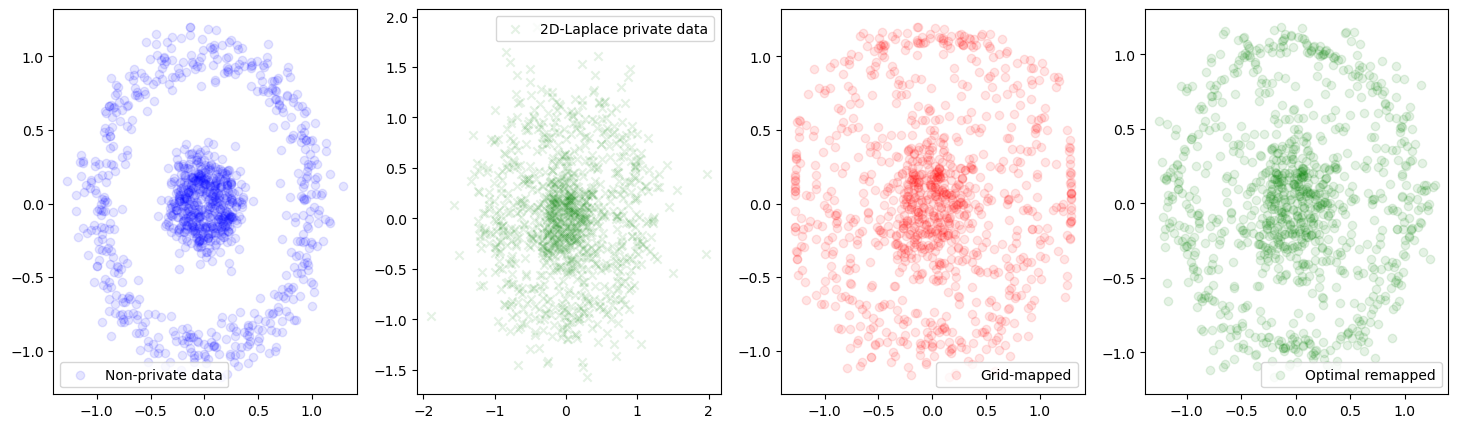
\includegraphics[width=1.1\textwidth]{TheorethicalFramework//ND-Laplace//Images/output.png}
  \caption{Example of optimal remapping for the 2-dimensional Circle dataset. The example shows the different steps of the mechanism in sequence for a dataset perturbed with a privacy budget of 0.5.}
\end{figure}
\begin{enumerate}
  \item Dataset: the blue dots represent the original dataset without any modifications.
  \item Adding noise: the green crosses represent the dataset after adding noise; for this particular example, this is 3D-Laplace (Algorithm \ref{alg:3d-laplace}):
        As can be observed, the data is generated from the center, causing many data points to fall outside the original domain of the dataset.
  \item Grid-remapping: the red dots represent the dataset after grid-remapping (Algorithm \ref{alg:grid-remapping-laplace})
        After performing the grid remapping algorithm, all points outside the data domain are remapped to be within the domain. The data-shape is also partly restored. 
  \item Optimal-remapping: the green dots represent the dataset after optimal-remapping (Algorithm \ref{alg:optimal-remapping-laplace}). As can be observed, this process is primarily on achieving a better utility by reproducing the original shape.
\end{enumerate}
